%!TEX root = presentation.tex
\section{Motivation}

\begin{frame}
	\frametitle{Big data analytics}
	\begin{columns}
		\begin{column}{0.6\textwidth}
			\begin{itemize}
				\item Gathered data grows exponentially
				\item Obtain new insights
				\item Analytic methods have to scale up $\Rightarrow$ Parallelization
				\item Methods developed within linear algebra systems
				\item Explicit parallelization tedious and error-prone
			\end{itemize}
		\end{column}
		\begin{column}{0.4\textwidth}
			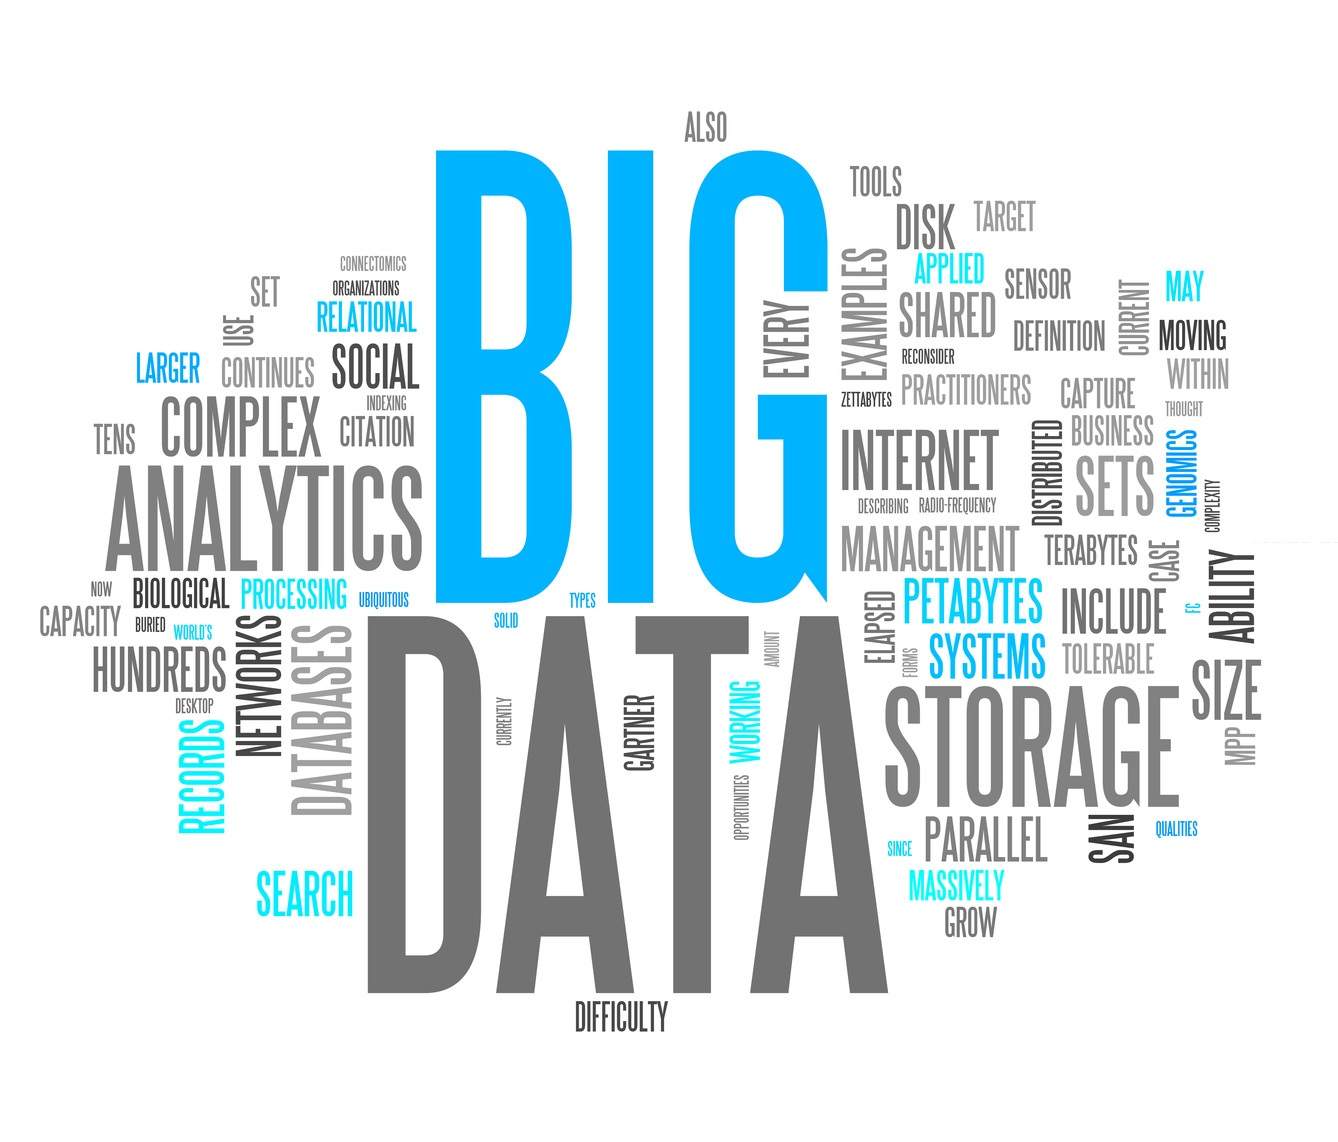
\includegraphics[width=\textwidth]{images/bigData.jpg}
		\end{column}
	\end{columns}
\end{frame}

\begin{frame}
	\frametitle{Distributed computing and data analytics}
	\begin{columns}
		\begin{column}{0.6\textwidth}
			\begin{itemize}
				\item Experts familiar with both domains countable
				\item Laborious to become acquainted with new domain
				\item Huge existing code base
				\item Can't we bring both worlds together?
				\item Solution: Gilbert
			\end{itemize}
		\end{column}
		\begin{column}{0.4\textwidth}
			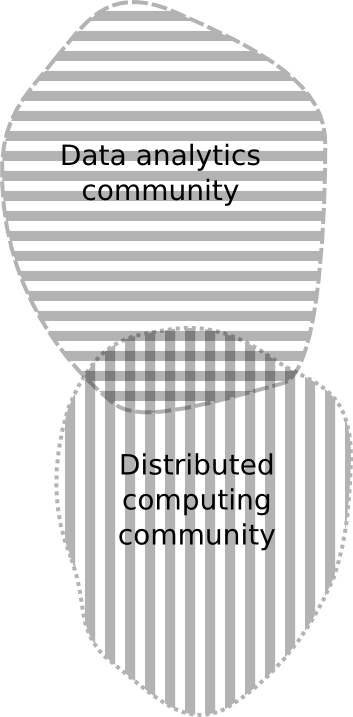
\includegraphics[height=0.8\textheight]{images/intersection.png}
		\end{column}
	\end{columns}
\end{frame}